%
\documentclass[12pt]{article}

% The usual packages
\usepackage{fullpage}
\usepackage{breakcites}
\usepackage{setspace}
\usepackage{endnotes}
\usepackage{float}
\usepackage{amsmath}
\usepackage{amsfonts}
\usepackage{amssymb}
\usepackage{rotating}
\usepackage{dcolumn}
\usepackage{longtable}
\usepackage{microtype}
\usepackage{graphicx}
\usepackage{hyperref}
%\usepackage[usenames,dvipsnames]{color}
\usepackage{url}
\usepackage{natbib}
\usepackage{framed}
\usepackage{epigraph}
\usepackage{lipsum}
\usepackage[font=small,labelfont=sc]{caption}
\restylefloat{table}
\bibpunct{(}{)}{;}{a}{}{,}

% Set paragraph spacing the way I like
\parskip=0pt
\parindent=20pt

% Define mathematical results
\newtheorem{lemma}{Lemma}
\newtheorem{proposition}{Proposition}
\newtheorem{theorem}{Theorem}
\newtheorem{claim}{Claim}
\newenvironment{proof}[1][Proof]{\begin{trivlist}
\item[\hskip \labelsep {\bfseries #1}]}{\end{trivlist}}
\newenvironment{definition}[1][Definition]{\begin{trivlist}
\item[\hskip \labelsep {\bfseries #1}]}{\end{trivlist}}
\newenvironment{example}[1][Example]{\begin{trivlist}
\item[\hskip \labelsep {\bfseries #1}]}{\end{trivlist}}
\newenvironment{remark}[1][Remark]{\begin{trivlist}
\item[\hskip \labelsep {\bfseries #1}]}{\end{trivlist}}

% Set up fonts the way I like
\usepackage{tgpagella}
\usepackage[T1]{fontenc}
\usepackage[bitstream-charter]{mathdesign}

%% Set up lists the way I like
% Redefine the first level
\renewcommand{\theenumi}{\arabic{enumi}.}
\renewcommand{\labelenumi}{\theenumi}
% Redefine the second level
\renewcommand{\theenumii}{\alph{enumii}.}
\renewcommand{\labelenumii}{\theenumii}
% Redefine the third level
\renewcommand{\theenumiii}{\roman{enumiii}.}
\renewcommand{\labelenumiii}{\theenumiii}
% Redefine the fourth level
\renewcommand{\theenumiv}{\Alph{enumiv}.}
\renewcommand{\labelenumiv}{\theenumiv}
% Eliminate spacing around lists
\usepackage{enumitem}
\setlist{nolistsep}

% Create footnote command so that my name
% has an asterisk rather than a one.
\long\def\symbolfootnote[#1]#2{\begingroup%
\def\thefootnote{\fnsymbol{footnote}}\footnote[#1]{#2}\endgroup}

% Create the colors I want
\usepackage{color}
\definecolor{darkred}{RGB}{100,0,0}

\hypersetup{
pdftitle={The Heavy Tails of Electoral Data}, % title
pdfauthor={Dan Baissa and Carlisle Rainey}, % author
pdfkeywords={robust linear regression} {outliers} {leverage}
pdfnewwindow=true, % links in new window
colorlinks=true, % false: boxed links; true: colored links
linkcolor=darkred, % color of internal links
citecolor=darkred, % color of links to bibliography
filecolor=darkred, % color of file links
urlcolor=darkred % color of external links
}

% enable comments in pdf
\newcommand{\kelly}[1]{\textcolor{blue}{#1}}
\newcommand{\carlisle}[1]{\textcolor{magenta}{#1}}


\begin{document}

\begin{center}
{\LARGE \textbf{The Heavy Tails of Electoral Data}}\\\vspace{2mm}
{ \textbf{The Importance of Robust Estimators}\symbolfootnote[1]{We thank Bill Clark and Matt Golder for making their data available to us. The analyses presented here were conducted with \texttt{R} 3.1.0. All data and computer code necessary for replication are available at \href{https://github.com/carlislerainey/heavy-tails}{
github.com/carlislerainey/meaningful-inferences}
.}}\\\vspace{2mm}


\vspace{10mm}

Dan Baissa\symbolfootnote[2]{Dan Baissa is an M.A. student in the Department of Political Science, University at Buffalo, SUNY, 520 Park Hall, Buffalo, NY 14260 (\href{mailto:dkbaissa@buffalo.edu}{
kellymcc@buffalo.edu}
).}

\vspace{3mm}

Carlisle Rainey\symbolfootnote[3]{Carlisle Rainey is Assistant Professor of Political Science, University at Buffalo, SUNY, 520 Park Hall, Buffalo, NY 14260 (\href{mailto:rcrainey@buffalo.edu}{
rcrainey@buffalo.edu}
).}
\end{center}

\vspace{10mm}

% Abstract
{\centerline{\textbf{Abstract}}}
\begin{quote}\noindent
Researchers studying the consequences of comparative electoral institutions, as well as other areas of political and social science, often estimate linear regression models on continuous outcomes of interest using least squares. These outcomes include measures of the number of political parties, proportionality, and vote share, among others. While it is well known that least-squares estimates are often sensitive to single, influential data point, this knowledge has not led to appropriate practices when using least-squares estimators. We highlight the important using more robust estimators (at least as a robustness check) and discuss several approaches to detect, summarize, and communicate the influence of particular data points. We conclude with a reanalysis of Clark and Golder (2006) an show that their conclusions depend on several influential data points. Removing these data or using a robust estimator substantially weaken their key conclusions about the conditional relationship between social heterogeneity and electoral rules in influencing the number of political parties.
 \end{quote}

% Add quote to first page
% \epigraph{}

%\begin{center}
%Manuscript word count: 
%\end{center}

% Remove page number from first page
\thispagestyle{empty}

% Start main text
\newpage
\doublespace

\section*{Introduction}


\singlespace
\bibliographystyle{apsr_fs}
%\bibliography{/Users/carlislerainey/Dropbox/papers/bibliography/bibliography.bib}
\bibliography{/Users/rcrainey/Dropbox/papers/bibliography/bibliography.bib}


\section*{Replication of Clark and Golder (2006)}

\begin{figure}[H]
\begin{center}
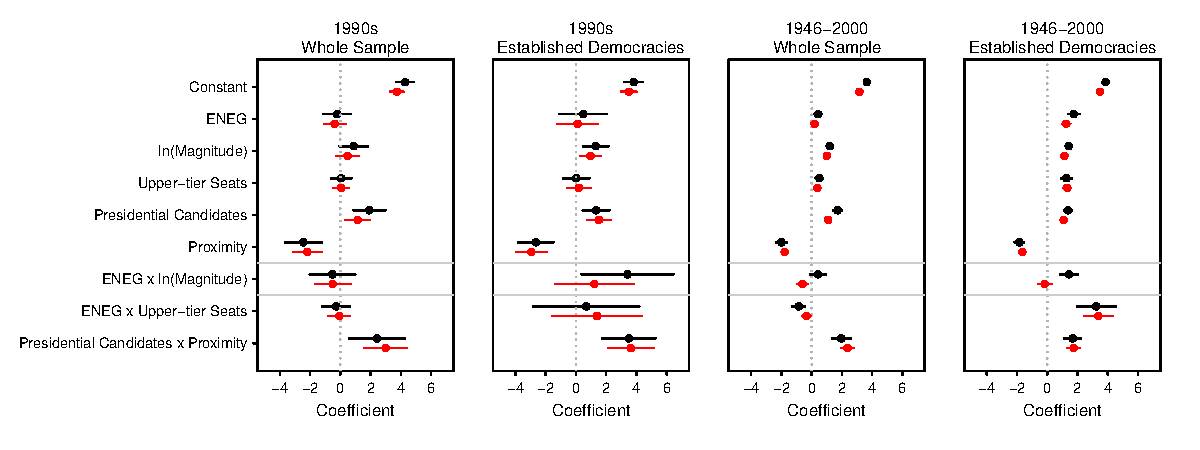
\includegraphics[scale = .8]{figs/cg-coef-plots.pdf}
\caption{Replication of Clark and Golder (2006) using MM-estimation with explanatory variables standardized to have mean zero and standard deviation one-half. The black lines and points show the OLS estimates and 90\% confidence intervals and the red lines and points show the MM estimates and confidence intervals. Notice that the coefficient for the product of the effective number of ethnic groups and the district magnitude changes drastically with the choice of estimator.}\label{fig:cg-coef-plots}
\end{center}
\end{figure}

\newpage
\doublespace
\begin{appendix}
\begin{center}
\textbf{{\LARGE Appendix}}\\\vspace{2mm}
\textbf{{\large The Heavy Tails of Electoral Data}}\\\vspace{2mm}

\end{center}
\section{}


\end{appendix}


\end{document}